\documentclass[11pt]{article}
\usepackage[margin=1in]{geometry}
\usepackage{amsmath,amssymb,amsthm}
\usepackage[T1]{fontenc}
\usepackage{lmodern}
\usepackage{microtype}
\usepackage{float}
\usepackage{pgfplots}
\usepgfplotslibrary{groupplots}
\pgfplotsset{compat=1.18}
\usepackage[hidelinks]{hyperref}
\setlength{\parindent}{0pt}
\setlength{\parskip}{0.55em}
\newtheorem{theorem}{Theorem}
\title{A Research Principle for the AI Era}
\author{Jianmin Liao}
\date{September 28, 2026}
\begin{document}
\maketitle

\textbf{Research in the AI era should pursue intrinsic value while building the external support needed to sustain that pursuit.}

Even when intrinsic value is the sole objective, an initial phase devoted entirely to external return can be necessary for optimal research. The model below makes this statement precise: with a sufficiently long horizon, every optimal strategy begins with full external focus, followed by an optimal phase that combines intrinsic work with the external return required to maintain a growing safety balance.

Here, intrinsic value means the scientific understanding or other substantive contribution that the researcher ultimately values. External return means support convertible into research funding, measured in the same units as expenditure. The distinction separates the purpose of research from the resources that sustain it.

\section*{Assumptions}

Consider a fixed number $n$ of research cycles. In cycle $i$, let $c_i$ be expenditure and $p_i\in[0,1]$ the share allocated to intrinsic work. Write $I_i$ and $E_i$ for intrinsic value and external return, respectively.

\textbf{1. Linear production and funding renewal.} Choose units so that $c_1=1$ and
\[
 I_i=p_i c_i,\qquad E_i=b(1-p_i)c_i,\qquad c_{i+1}=E_i.
\]
The first two relations give a constant return per unit allocated to either activity. The third makes the next cycle's research budget equal to the current external return. For the final cycle, $c_{n+1}$ is only a convenient name for $E_n$.

\textbf{2. A positive and growing safety balance.} Let $B_i$ denote the cumulative funding surplus at the end of cycle $i$:
\[
 B_0=0,\qquad B_i=B_{i-1}+E_i-c_i.
\]
Require
\[
 B_i\ge\max\{\delta,\rho B_{i-1}\},\qquad
 0<\delta\le b-1,\qquad 1<\rho<b.
\]
The fixed floor $\delta$ establishes a safety reserve, while $\rho$ requires it to grow. The upper bound on $\delta$ makes the first cycle feasible. The inequality $\rho<b$ leaves room to produce intrinsic value while meeting the growth requirement. Funding is assessed at cycle boundaries; the initial expenditure is supplied as seed funding.

\textbf{3. Intrinsic value as the sole objective.} Choose the allocation shares to maximize
\[
 \sum_{i=1}^{n} I_i.
\]
Returns are deterministic, each cycle's intrinsic value receives equal weight, and external return has value through the funding dynamics and constraints.

\textbf{4. Enough time for reinvestment.} Define
\[
 K=\min\left\{m\ge1:(b-\rho)\sum_{j=0}^{m-1}\rho^j>1\right\},
 \qquad n>K.
\]
Here $m$ is an integer. Since $b>\rho>1$, $K$ is finite. This assumption gives early external returns enough time to generate later intrinsic value.

\section*{Result}

\begin{theorem}
Under these assumptions, every optimal strategy devotes the first $n-K$ cycles entirely to external return:
\[
 p_i=0\qquad (1\le i\le n-K).
\]
There is an optimal strategy that then meets the balance-growth constraint exactly in all remaining cycles:
\[
 B_i=\rho B_{i-1},\qquad
 p_i=1-\frac{1+\rho B_{i-1}}{b(1+B_{i-1})}\in(0,1)
 \qquad(n-K<i\le n).
\]
Thus, maximizing intrinsic value alone requires an initial phase of full external focus and admits a single subsequent switch to a mixture of intrinsic and external work.
\end{theorem}

\section*{A numerical example}

\begin{figure}[H]
\centering
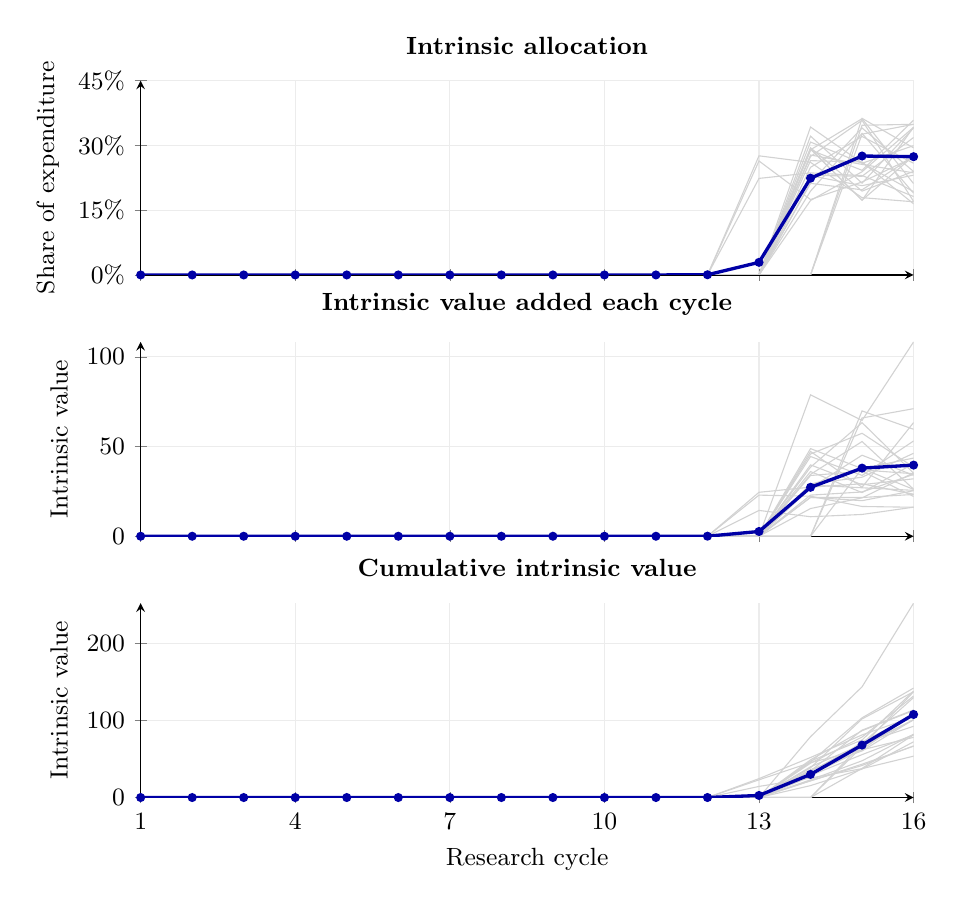
\begin{tikzpicture}
\begin{groupplot}[group style={group size=1 by 3,vertical sep=0.85cm},
width=0.94\textwidth,height=4.05cm,xmin=1,xmax=16,ymin=0,
xtick={1,4,7,10,13,16},grid=major,grid style={gray!15},
axis lines=left,tick label style={font=\small},label style={font=\small},
title style={font=\small\bfseries},scaled y ticks=false]
\nextgroupplot[title={Intrinsic allocation},ylabel={Share of expenditure},xticklabels={},ymax=45,ytick={0,15,30,45},yticklabel={\pgfmathprintnumber{\tick}\%}]
\addplot[gray!35,thin] coordinates {(1,0.00000) (2,0.00000) (3,0.00000) (4,0.00000) (5,0.00000) (6,0.00000) (7,0.00000) (8,0.00000) (9,0.00000) (10,0.00000) (11,0.00000) (12,0.00000) (13,0.00000) (14,19.40786) (15,32.77975) (16,18.93779)};
\addplot[gray!35,thin] coordinates {(1,0.00000) (2,0.00000) (3,0.00000) (4,0.00000) (5,0.00000) (6,0.00000) (7,0.00000) (8,0.00000) (9,0.00000) (10,0.00000) (11,0.00000) (12,0.00000) (13,0.00000) (14,26.46255) (15,26.15191) (16,16.46312)};
\addplot[gray!35,thin] coordinates {(1,0.00000) (2,0.00000) (3,0.00000) (4,0.00000) (5,0.00000) (6,0.00000) (7,0.00000) (8,0.00000) (9,0.00000) (10,0.00000) (11,0.00000) (12,0.00000) (13,0.00000) (14,32.14430) (15,21.24931) (16,34.02903)};
\addplot[gray!35,thin] coordinates {(1,0.00000) (2,0.00000) (3,0.00000) (4,0.00000) (5,0.00000) (6,0.00000) (7,0.00000) (8,0.00000) (9,0.00000) (10,0.00000) (11,0.00000) (12,0.00000) (13,0.00000) (14,23.07189) (15,22.84563) (16,31.82748)};
\addplot[gray!35,thin] coordinates {(1,0.00000) (2,0.00000) (3,0.00000) (4,0.00000) (5,0.00000) (6,0.00000) (7,0.00000) (8,0.00000) (9,0.00000) (10,0.00000) (11,0.00000) (12,0.00000) (13,0.00000) (14,27.76794) (15,25.59004) (16,23.62704)};
\addplot[gray!35,thin] coordinates {(1,0.00000) (2,0.00000) (3,0.00000) (4,0.00000) (5,0.00000) (6,0.00000) (7,0.00000) (8,0.00000) (9,0.00000) (10,0.00000) (11,0.00000) (12,0.00000) (13,0.00000) (14,0.00000) (15,34.65974) (16,34.86800)};
\addplot[gray!35,thin] coordinates {(1,0.00000) (2,0.00000) (3,0.00000) (4,0.00000) (5,0.00000) (6,0.00000) (7,0.00000) (8,0.00000) (9,0.00000) (10,0.00000) (11,0.00000) (12,0.00000) (13,0.00000) (14,0.00000) (15,32.59946) (16,34.87102)};
\addplot[gray!35,thin] coordinates {(1,0.00000) (2,0.00000) (3,0.00000) (4,0.00000) (5,0.00000) (6,0.00000) (7,0.00000) (8,0.00000) (9,0.00000) (10,0.00000) (11,0.00000) (12,0.00000) (13,26.38904) (14,17.46043) (15,21.51735) (16,27.23394)};
\addplot[gray!35,thin] coordinates {(1,0.00000) (2,0.00000) (3,0.00000) (4,0.00000) (5,0.00000) (6,0.00000) (7,0.00000) (8,0.00000) (9,0.00000) (10,0.00000) (11,0.00000) (12,0.00000) (13,0.00000) (14,27.42527) (15,35.79980) (16,17.03286)};
\addplot[gray!35,thin] coordinates {(1,0.00000) (2,0.00000) (3,0.00000) (4,0.00000) (5,0.00000) (6,0.00000) (7,0.00000) (8,0.00000) (9,0.00000) (10,0.00000) (11,0.00000) (12,0.00000) (13,0.00000) (14,30.76572) (15,25.85786) (16,29.93400)};
\addplot[gray!35,thin] coordinates {(1,0.00000) (2,0.00000) (3,0.00000) (4,0.00000) (5,0.00000) (6,0.00000) (7,0.00000) (8,0.00000) (9,0.00000) (10,0.00000) (11,0.00000) (12,0.00000) (13,0.00000) (14,34.24370) (15,25.93172) (16,19.27721)};
\addplot[gray!35,thin] coordinates {(1,0.00000) (2,0.00000) (3,0.00000) (4,0.00000) (5,0.00000) (6,0.00000) (7,0.00000) (8,0.00000) (9,0.00000) (10,0.00000) (11,0.00000) (12,0.00000) (13,0.00000) (14,17.23491) (15,23.89738) (16,34.18335)};
\addplot[gray!35,thin] coordinates {(1,0.00000) (2,0.00000) (3,0.00000) (4,0.00000) (5,0.00000) (6,0.00000) (7,0.00000) (8,0.00000) (9,0.00000) (10,0.00000) (11,0.00000) (12,0.00000) (13,0.00000) (14,28.98358) (15,36.17819) (16,21.13706)};
\addplot[gray!35,thin] coordinates {(1,0.00000) (2,0.00000) (3,0.00000) (4,0.00000) (5,0.00000) (6,0.00000) (7,0.00000) (8,0.00000) (9,0.00000) (10,0.00000) (11,0.00000) (12,0.00000) (13,0.00000) (14,29.25626) (15,17.29095) (16,34.25296)};
\addplot[gray!35,thin] coordinates {(1,0.00000) (2,0.00000) (3,0.00000) (4,0.00000) (5,0.00000) (6,0.00000) (7,0.00000) (8,0.00000) (9,0.00000) (10,0.00000) (11,0.00000) (12,0.00000) (13,22.35057) (14,23.63032) (15,23.01605) (16,18.15591)};
\addplot[gray!35,thin] coordinates {(1,0.00000) (2,0.00000) (3,0.00000) (4,0.00000) (5,0.00000) (6,0.00000) (7,0.00000) (8,0.00000) (9,0.00000) (10,0.00000) (11,0.00000) (12,0.00000) (13,0.00000) (14,0.00000) (15,36.25671) (16,29.41136)};
\addplot[gray!35,thin] coordinates {(1,0.00000) (2,0.00000) (3,0.00000) (4,0.00000) (5,0.00000) (6,0.00000) (7,0.00000) (8,0.00000) (9,0.00000) (10,0.00000) (11,0.00000) (12,0.00000) (13,27.57634) (14,26.05855) (15,17.89287) (16,16.94074)};
\addplot[gray!35,thin] coordinates {(1,0.00000) (2,0.00000) (3,0.00000) (4,0.00000) (5,0.00000) (6,0.00000) (7,0.00000) (8,0.00000) (9,0.00000) (10,0.00000) (11,0.00000) (12,0.00000) (13,0.00000) (14,29.09613) (15,17.31227) (16,27.52694)};
\addplot[gray!35,thin] coordinates {(1,0.00000) (2,0.00000) (3,0.00000) (4,0.00000) (5,0.00000) (6,0.00000) (7,0.00000) (8,0.00000) (9,0.00000) (10,0.00000) (11,0.00000) (12,0.00000) (13,0.00000) (14,21.20670) (15,19.70865) (16,27.41671)};
\addplot[gray!35,thin] coordinates {(1,0.00000) (2,0.00000) (3,0.00000) (4,0.00000) (5,0.00000) (6,0.00000) (7,0.00000) (8,0.00000) (9,0.00000) (10,0.00000) (11,0.00000) (12,0.00000) (13,0.00000) (14,21.40642) (15,34.02087) (16,23.95204)};
\addplot[gray!35,thin] coordinates {(1,0.00000) (2,0.00000) (3,0.00000) (4,0.00000) (5,0.00000) (6,0.00000) (7,0.00000) (8,0.00000) (9,0.00000) (10,0.00000) (11,0.00000) (12,0.00000) (13,0.00000) (14,24.92532) (15,32.06591) (16,25.85515)};
\addplot[gray!35,thin] coordinates {(1,0.00000) (2,0.00000) (3,0.00000) (4,0.00000) (5,0.00000) (6,0.00000) (7,0.00000) (8,0.00000) (9,0.00000) (10,0.00000) (11,0.00000) (12,0.00000) (13,0.00000) (14,29.44285) (15,19.40932) (16,23.97408)};
\addplot[gray!35,thin] coordinates {(1,0.00000) (2,0.00000) (3,0.00000) (4,0.00000) (5,0.00000) (6,0.00000) (7,0.00000) (8,0.00000) (9,0.00000) (10,0.00000) (11,0.00000) (12,0.00000) (13,0.00000) (14,22.96539) (15,20.66828) (16,23.10177)};
\addplot[gray!35,thin] coordinates {(1,0.00000) (2,0.00000) (3,0.00000) (4,0.00000) (5,0.00000) (6,0.00000) (7,0.00000) (8,0.00000) (9,0.00000) (10,0.00000) (11,0.00000) (12,0.00000) (13,0.00000) (14,28.91523) (15,24.22614) (16,35.82776)};
\addplot[blue!65!black,very thick,mark=*,mark size=1pt] coordinates {(1,0.00000) (2,0.00000) (3,0.00000) (4,0.00000) (5,0.00000) (6,0.00000) (7,0.00000) (8,0.00000) (9,0.00000) (10,0.00000) (11,0.00000) (12,0.04102) (13,2.91631) (14,22.40419) (15,27.53240) (16,27.37889)};
\nextgroupplot[title={Intrinsic value added each cycle},ylabel={Intrinsic value},xticklabels={}]
\addplot[gray!35,thin] coordinates {(1,0.00000) (2,0.00000) (3,0.00000) (4,0.00000) (5,0.00000) (6,0.00000) (7,0.00000) (8,0.00000) (9,0.00000) (10,0.00000) (11,0.00000) (12,0.00000) (13,0.00000) (14,38.51710) (15,63.34597) (16,35.13974)};
\addplot[gray!35,thin] coordinates {(1,0.00000) (2,0.00000) (3,0.00000) (4,0.00000) (5,0.00000) (6,0.00000) (7,0.00000) (8,0.00000) (9,0.00000) (10,0.00000) (11,0.00000) (12,0.00000) (13,0.00000) (14,33.85897) (15,36.25858) (16,22.20212)};
\addplot[gray!35,thin] coordinates {(1,0.00000) (2,0.00000) (3,0.00000) (4,0.00000) (5,0.00000) (6,0.00000) (7,0.00000) (8,0.00000) (9,0.00000) (10,0.00000) (11,0.00000) (12,0.00000) (13,0.00000) (14,44.45225) (15,33.92879) (16,53.13501)};
\addplot[gray!35,thin] coordinates {(1,0.00000) (2,0.00000) (3,0.00000) (4,0.00000) (5,0.00000) (6,0.00000) (7,0.00000) (8,0.00000) (9,0.00000) (10,0.00000) (11,0.00000) (12,0.00000) (13,0.00000) (14,29.17747) (15,32.92242) (16,46.27670)};
\addplot[gray!35,thin] coordinates {(1,0.00000) (2,0.00000) (3,0.00000) (4,0.00000) (5,0.00000) (6,0.00000) (7,0.00000) (8,0.00000) (9,0.00000) (10,0.00000) (11,0.00000) (12,0.00000) (13,0.00000) (14,28.56843) (15,27.02560) (16,25.60046)};
\addplot[gray!35,thin] coordinates {(1,0.00000) (2,0.00000) (3,0.00000) (4,0.00000) (5,0.00000) (6,0.00000) (7,0.00000) (8,0.00000) (9,0.00000) (10,0.00000) (11,0.00000) (12,0.00000) (13,0.00000) (14,0.00000) (15,37.73799) (16,43.59511)};
\addplot[gray!35,thin] coordinates {(1,0.00000) (2,0.00000) (3,0.00000) (4,0.00000) (5,0.00000) (6,0.00000) (7,0.00000) (8,0.00000) (9,0.00000) (10,0.00000) (11,0.00000) (12,0.00000) (13,0.00000) (14,0.00000) (15,65.94976) (16,71.13947)};
\addplot[gray!35,thin] coordinates {(1,0.00000) (2,0.00000) (3,0.00000) (4,0.00000) (5,0.00000) (6,0.00000) (7,0.00000) (8,0.00000) (9,0.00000) (10,0.00000) (11,0.00000) (12,0.00000) (13,14.39322) (14,10.87832) (15,12.14973) (16,16.21665)};
\addplot[gray!35,thin] coordinates {(1,0.00000) (2,0.00000) (3,0.00000) (4,0.00000) (5,0.00000) (6,0.00000) (7,0.00000) (8,0.00000) (9,0.00000) (10,0.00000) (11,0.00000) (12,0.00000) (13,0.00000) (14,34.48355) (15,52.81665) (16,26.22469)};
\addplot[gray!35,thin] coordinates {(1,0.00000) (2,0.00000) (3,0.00000) (4,0.00000) (5,0.00000) (6,0.00000) (7,0.00000) (8,0.00000) (9,0.00000) (10,0.00000) (11,0.00000) (12,0.00000) (13,0.00000) (14,21.70571) (15,19.83002) (16,25.39030)};
\addplot[gray!35,thin] coordinates {(1,0.00000) (2,0.00000) (3,0.00000) (4,0.00000) (5,0.00000) (6,0.00000) (7,0.00000) (8,0.00000) (9,0.00000) (10,0.00000) (11,0.00000) (12,0.00000) (13,0.00000) (14,48.86872) (15,37.70855) (16,26.13513)};
\addplot[gray!35,thin] coordinates {(1,0.00000) (2,0.00000) (3,0.00000) (4,0.00000) (5,0.00000) (6,0.00000) (7,0.00000) (8,0.00000) (9,0.00000) (10,0.00000) (11,0.00000) (12,0.00000) (13,0.00000) (14,15.44813) (15,21.41250) (16,35.34447)};
\addplot[gray!35,thin] coordinates {(1,0.00000) (2,0.00000) (3,0.00000) (4,0.00000) (5,0.00000) (6,0.00000) (7,0.00000) (8,0.00000) (9,0.00000) (10,0.00000) (11,0.00000) (12,0.00000) (13,0.00000) (14,45.86716) (15,57.40593) (16,38.54708)};
\addplot[gray!35,thin] coordinates {(1,0.00000) (2,0.00000) (3,0.00000) (4,0.00000) (5,0.00000) (6,0.00000) (7,0.00000) (8,0.00000) (9,0.00000) (10,0.00000) (11,0.00000) (12,0.00000) (13,0.00000) (14,47.26595) (15,27.32403) (16,63.39576)};
\addplot[gray!35,thin] coordinates {(1,0.00000) (2,0.00000) (3,0.00000) (4,0.00000) (5,0.00000) (6,0.00000) (7,0.00000) (8,0.00000) (9,0.00000) (10,0.00000) (11,0.00000) (12,0.00000) (13,24.50637) (14,27.38148) (15,29.25349) (16,23.42986)};
\addplot[gray!35,thin] coordinates {(1,0.00000) (2,0.00000) (3,0.00000) (4,0.00000) (5,0.00000) (6,0.00000) (7,0.00000) (8,0.00000) (9,0.00000) (10,0.00000) (11,0.00000) (12,0.00000) (13,0.00000) (14,0.00000) (15,69.88397) (16,59.64794)};
\addplot[gray!35,thin] coordinates {(1,0.00000) (2,0.00000) (3,0.00000) (4,0.00000) (5,0.00000) (6,0.00000) (7,0.00000) (8,0.00000) (9,0.00000) (10,0.00000) (11,0.00000) (12,0.00000) (13,22.93127) (14,22.32292) (15,16.59871) (16,16.16071)};
\addplot[gray!35,thin] coordinates {(1,0.00000) (2,0.00000) (3,0.00000) (4,0.00000) (5,0.00000) (6,0.00000) (7,0.00000) (8,0.00000) (9,0.00000) (10,0.00000) (11,0.00000) (12,0.00000) (13,0.00000) (14,36.07158) (15,24.35317) (16,40.54784)};
\addplot[gray!35,thin] coordinates {(1,0.00000) (2,0.00000) (3,0.00000) (4,0.00000) (5,0.00000) (6,0.00000) (7,0.00000) (8,0.00000) (9,0.00000) (10,0.00000) (11,0.00000) (12,0.00000) (13,0.00000) (14,22.92945) (15,24.68159) (16,34.47777)};
\addplot[gray!35,thin] coordinates {(1,0.00000) (2,0.00000) (3,0.00000) (4,0.00000) (5,0.00000) (6,0.00000) (7,0.00000) (8,0.00000) (9,0.00000) (10,0.00000) (11,0.00000) (12,0.00000) (13,0.00000) (14,26.92210) (15,45.18179) (16,34.00468)};
\addplot[gray!35,thin] coordinates {(1,0.00000) (2,0.00000) (3,0.00000) (4,0.00000) (5,0.00000) (6,0.00000) (7,0.00000) (8,0.00000) (9,0.00000) (10,0.00000) (11,0.00000) (12,0.00000) (13,0.00000) (14,28.93348) (15,36.96905) (16,34.86305)};
\addplot[gray!35,thin] coordinates {(1,0.00000) (2,0.00000) (3,0.00000) (4,0.00000) (5,0.00000) (6,0.00000) (7,0.00000) (8,0.00000) (9,0.00000) (10,0.00000) (11,0.00000) (12,0.00000) (13,0.00000) (14,39.79105) (15,28.72943) (16,32.02925)};
\addplot[gray!35,thin] coordinates {(1,0.00000) (2,0.00000) (3,0.00000) (4,0.00000) (5,0.00000) (6,0.00000) (7,0.00000) (8,0.00000) (9,0.00000) (10,0.00000) (11,0.00000) (12,0.00000) (13,0.00000) (14,21.62019) (15,21.60107) (16,23.30667)};
\addplot[gray!35,thin] coordinates {(1,0.00000) (2,0.00000) (3,0.00000) (4,0.00000) (5,0.00000) (6,0.00000) (7,0.00000) (8,0.00000) (9,0.00000) (10,0.00000) (11,0.00000) (12,0.00000) (13,0.00000) (14,78.84157) (15,64.59257) (16,108.38799)};
\addplot[blue!65!black,very thick,mark=*,mark size=1pt] coordinates {(1,0.00000) (2,0.00000) (3,0.00000) (4,0.00000) (5,0.00000) (6,0.00000) (7,0.00000) (8,0.00000) (9,0.00000) (10,0.00000) (11,0.00000) (12,0.03490) (13,2.64724) (14,27.29894) (15,37.98646) (16,39.66623)};
\nextgroupplot[title={Cumulative intrinsic value},ylabel={Intrinsic value},xlabel={Research cycle}]
\addplot[gray!35,thin] coordinates {(1,0.00000) (2,0.00000) (3,0.00000) (4,0.00000) (5,0.00000) (6,0.00000) (7,0.00000) (8,0.00000) (9,0.00000) (10,0.00000) (11,0.00000) (12,0.00000) (13,0.00000) (14,38.51710) (15,101.86307) (16,137.00282)};
\addplot[gray!35,thin] coordinates {(1,0.00000) (2,0.00000) (3,0.00000) (4,0.00000) (5,0.00000) (6,0.00000) (7,0.00000) (8,0.00000) (9,0.00000) (10,0.00000) (11,0.00000) (12,0.00000) (13,0.00000) (14,33.85897) (15,70.11754) (16,92.31966)};
\addplot[gray!35,thin] coordinates {(1,0.00000) (2,0.00000) (3,0.00000) (4,0.00000) (5,0.00000) (6,0.00000) (7,0.00000) (8,0.00000) (9,0.00000) (10,0.00000) (11,0.00000) (12,0.00000) (13,0.00000) (14,44.45225) (15,78.38104) (16,131.51605)};
\addplot[gray!35,thin] coordinates {(1,0.00000) (2,0.00000) (3,0.00000) (4,0.00000) (5,0.00000) (6,0.00000) (7,0.00000) (8,0.00000) (9,0.00000) (10,0.00000) (11,0.00000) (12,0.00000) (13,0.00000) (14,29.17747) (15,62.09989) (16,108.37659)};
\addplot[gray!35,thin] coordinates {(1,0.00000) (2,0.00000) (3,0.00000) (4,0.00000) (5,0.00000) (6,0.00000) (7,0.00000) (8,0.00000) (9,0.00000) (10,0.00000) (11,0.00000) (12,0.00000) (13,0.00000) (14,28.56843) (15,55.59403) (16,81.19449)};
\addplot[gray!35,thin] coordinates {(1,0.00000) (2,0.00000) (3,0.00000) (4,0.00000) (5,0.00000) (6,0.00000) (7,0.00000) (8,0.00000) (9,0.00000) (10,0.00000) (11,0.00000) (12,0.00000) (13,0.00000) (14,0.00000) (15,37.73799) (16,81.33310)};
\addplot[gray!35,thin] coordinates {(1,0.00000) (2,0.00000) (3,0.00000) (4,0.00000) (5,0.00000) (6,0.00000) (7,0.00000) (8,0.00000) (9,0.00000) (10,0.00000) (11,0.00000) (12,0.00000) (13,0.00000) (14,0.00000) (15,65.94976) (16,137.08923)};
\addplot[gray!35,thin] coordinates {(1,0.00000) (2,0.00000) (3,0.00000) (4,0.00000) (5,0.00000) (6,0.00000) (7,0.00000) (8,0.00000) (9,0.00000) (10,0.00000) (11,0.00000) (12,0.00000) (13,14.39322) (14,25.27154) (15,37.42127) (16,53.63791)};
\addplot[gray!35,thin] coordinates {(1,0.00000) (2,0.00000) (3,0.00000) (4,0.00000) (5,0.00000) (6,0.00000) (7,0.00000) (8,0.00000) (9,0.00000) (10,0.00000) (11,0.00000) (12,0.00000) (13,0.00000) (14,34.48355) (15,87.30020) (16,113.52489)};
\addplot[gray!35,thin] coordinates {(1,0.00000) (2,0.00000) (3,0.00000) (4,0.00000) (5,0.00000) (6,0.00000) (7,0.00000) (8,0.00000) (9,0.00000) (10,0.00000) (11,0.00000) (12,0.00000) (13,0.00000) (14,21.70571) (15,41.53573) (16,66.92603)};
\addplot[gray!35,thin] coordinates {(1,0.00000) (2,0.00000) (3,0.00000) (4,0.00000) (5,0.00000) (6,0.00000) (7,0.00000) (8,0.00000) (9,0.00000) (10,0.00000) (11,0.00000) (12,0.00000) (13,0.00000) (14,48.86872) (15,86.57727) (16,112.71240)};
\addplot[gray!35,thin] coordinates {(1,0.00000) (2,0.00000) (3,0.00000) (4,0.00000) (5,0.00000) (6,0.00000) (7,0.00000) (8,0.00000) (9,0.00000) (10,0.00000) (11,0.00000) (12,0.00000) (13,0.00000) (14,15.44813) (15,36.86063) (16,72.20510)};
\addplot[gray!35,thin] coordinates {(1,0.00000) (2,0.00000) (3,0.00000) (4,0.00000) (5,0.00000) (6,0.00000) (7,0.00000) (8,0.00000) (9,0.00000) (10,0.00000) (11,0.00000) (12,0.00000) (13,0.00000) (14,45.86716) (15,103.27309) (16,141.82017)};
\addplot[gray!35,thin] coordinates {(1,0.00000) (2,0.00000) (3,0.00000) (4,0.00000) (5,0.00000) (6,0.00000) (7,0.00000) (8,0.00000) (9,0.00000) (10,0.00000) (11,0.00000) (12,0.00000) (13,0.00000) (14,47.26595) (15,74.58998) (16,137.98574)};
\addplot[gray!35,thin] coordinates {(1,0.00000) (2,0.00000) (3,0.00000) (4,0.00000) (5,0.00000) (6,0.00000) (7,0.00000) (8,0.00000) (9,0.00000) (10,0.00000) (11,0.00000) (12,0.00000) (13,24.50637) (14,51.88785) (15,81.14134) (16,104.57120)};
\addplot[gray!35,thin] coordinates {(1,0.00000) (2,0.00000) (3,0.00000) (4,0.00000) (5,0.00000) (6,0.00000) (7,0.00000) (8,0.00000) (9,0.00000) (10,0.00000) (11,0.00000) (12,0.00000) (13,0.00000) (14,0.00000) (15,69.88397) (16,129.53191)};
\addplot[gray!35,thin] coordinates {(1,0.00000) (2,0.00000) (3,0.00000) (4,0.00000) (5,0.00000) (6,0.00000) (7,0.00000) (8,0.00000) (9,0.00000) (10,0.00000) (11,0.00000) (12,0.00000) (13,22.93127) (14,45.25418) (15,61.85290) (16,78.01360)};
\addplot[gray!35,thin] coordinates {(1,0.00000) (2,0.00000) (3,0.00000) (4,0.00000) (5,0.00000) (6,0.00000) (7,0.00000) (8,0.00000) (9,0.00000) (10,0.00000) (11,0.00000) (12,0.00000) (13,0.00000) (14,36.07158) (15,60.42476) (16,100.97260)};
\addplot[gray!35,thin] coordinates {(1,0.00000) (2,0.00000) (3,0.00000) (4,0.00000) (5,0.00000) (6,0.00000) (7,0.00000) (8,0.00000) (9,0.00000) (10,0.00000) (11,0.00000) (12,0.00000) (13,0.00000) (14,22.92945) (15,47.61103) (16,82.08880)};
\addplot[gray!35,thin] coordinates {(1,0.00000) (2,0.00000) (3,0.00000) (4,0.00000) (5,0.00000) (6,0.00000) (7,0.00000) (8,0.00000) (9,0.00000) (10,0.00000) (11,0.00000) (12,0.00000) (13,0.00000) (14,26.92210) (15,72.10389) (16,106.10857)};
\addplot[gray!35,thin] coordinates {(1,0.00000) (2,0.00000) (3,0.00000) (4,0.00000) (5,0.00000) (6,0.00000) (7,0.00000) (8,0.00000) (9,0.00000) (10,0.00000) (11,0.00000) (12,0.00000) (13,0.00000) (14,28.93348) (15,65.90253) (16,100.76558)};
\addplot[gray!35,thin] coordinates {(1,0.00000) (2,0.00000) (3,0.00000) (4,0.00000) (5,0.00000) (6,0.00000) (7,0.00000) (8,0.00000) (9,0.00000) (10,0.00000) (11,0.00000) (12,0.00000) (13,0.00000) (14,39.79105) (15,68.52049) (16,100.54973)};
\addplot[gray!35,thin] coordinates {(1,0.00000) (2,0.00000) (3,0.00000) (4,0.00000) (5,0.00000) (6,0.00000) (7,0.00000) (8,0.00000) (9,0.00000) (10,0.00000) (11,0.00000) (12,0.00000) (13,0.00000) (14,21.62019) (15,43.22126) (16,66.52792)};
\addplot[gray!35,thin] coordinates {(1,0.00000) (2,0.00000) (3,0.00000) (4,0.00000) (5,0.00000) (6,0.00000) (7,0.00000) (8,0.00000) (9,0.00000) (10,0.00000) (11,0.00000) (12,0.00000) (13,0.00000) (14,78.84157) (15,143.43415) (16,251.82214)};
\addplot[blue!65!black,very thick,mark=*,mark size=1pt] coordinates {(1,0.00000) (2,0.00000) (3,0.00000) (4,0.00000) (5,0.00000) (6,0.00000) (7,0.00000) (8,0.00000) (9,0.00000) (10,0.00000) (11,0.00000) (12,0.03490) (13,2.68214) (14,29.98108) (15,67.96755) (16,107.63377)};
\end{groupplot}
\end{tikzpicture}
\caption{Changing return functions across cycles. Thin lines show the first 24 of 400 optimized scenarios; thick lines show the mean over all 400. Panels show the intrinsic allocation share, the intrinsic value added in each cycle, and cumulative intrinsic value. Each scenario changes both return slopes in every cycle.}
\end{figure}

We optimize 400 scenarios with $n=16$, $\rho=1.05$, and $\delta=0.1$. Within each scenario, both return functions change in every cycle:
\[
 I_i=a_i p_i c_i,\qquad E_i=b_i(1-p_i)c_i,
\]
\[
 0.9\le a_i\le1.1,\qquad 1.25\le b_i\le1.65,\qquad c_{i+1}=E_i.
\]
The slopes are sampled independently and uniformly within these intervals, using seed 20260928. Each complete sequence is known when its optimal allocation is computed by backward induction. The initial expenditure and balance rules are as above.

For every sequence within these bounds, the argument below guarantees full external focus for at least the first ten cycles and an optimal single switch to mixed allocation. In the 400 simulated scenarios, this initial phase lasts 11--14 cycles. By cycle 16, the mean intrinsic allocation is 27.4\%, the mean intrinsic increment is 39.67, and the mean cumulative intrinsic value is 107.63 in normalized intrinsic-value units. The plotted averages include all 400 scenarios in every cycle.

\section*{Proof}

The funding identity telescopes to
\[
 B_i=c_{i+1}-1,\qquad c_i=1+B_{i-1}.
\]
Consequently, at any cycle after the first, a current balance $B\ge\delta$ permits exactly the next balances $B'$ satisfying
\[
 \rho B\le B'\le bB+b-1.
\]
The intrinsic value earned in that cycle is
\[
 I=1-\frac1b+B-\frac{B'}b.
\]
The upper endpoint corresponds to $p=0$; the lower endpoint meets the required balance growth exactly.

Let $V_m(B)$ be the largest total intrinsic value attainable with $m$ cycles remaining and current balance $B\ge\delta$. We show by induction that $V_m$ is affine in $B$, and denote its slope by $A_m$. Since $V_0=0$, $A_0=0$. The recursion is
\[
 V_m(B)=1-\frac1b+B+
 \max_{\rho B\le B'\le bB+b-1}
 \left\{V_{m-1}(B')-\frac{B'}b\right\}.
\]
If $V_{m-1}$ is affine, the coefficient of $B'$ is $A_{m-1}-1/b$. Therefore the maximizing choice is the upper endpoint when $A_{m-1}>1/b$, and the lower endpoint when $A_{m-1}<1/b$. At equality, either endpoint is optimal; choose the lower one. Substitution shows that $V_m$ is affine and gives
\[
 A_m=
 \begin{cases}
 1-\rho/b+\rho A_{m-1},&A_{m-1}\le1/b,\\
 bA_{m-1},&A_{m-1}>1/b.
 \end{cases}
\]
Until the threshold is crossed,
\[
 A_m=\frac{b-\rho}{b}\sum_{j=0}^{m-1}\rho^j.
\]
Hence $A_{K-1}\le1/b<A_K$. After this crossing, the second branch keeps $A_m>1/b$. It follows that every cycle with more than $K$ cycles remaining has the unique optimal choice of full external focus. With at most $K$ cycles remaining, choosing the lower endpoint is optimal.

For the first cycle, the feasible interval is $\delta\le B_1\le b-1$. Its objective has coefficient $A_{n-1}-1/b$ on $B_1$. Since $n>K$, this coefficient is strictly positive, so every optimum chooses $B_1=b-1$, equivalently $p_1=0$. The same argument applies to the subsequent cycles with more than $K$ cycles remaining.

In the last $K$ cycles, choose $B_i=\rho B_{i-1}$. The formula for $p_i$ follows from $E_i=1+B_i=b(1-p_i)(1+B_{i-1})$. Since $B_{i-1}>0$ and $1<\rho<b$, this share lies strictly between zero and one. This proves the result.\hfill$\square$

\textbf{Extension to the changing functions in the example.}
For cycles after the first, the same balance identity and feasible interval apply with the current $b_i$. Let $A$ be the slope of the continuation value. The coefficient of the next balance is now $A-a_i/b_i$: choose the upper endpoint when it is positive, and the lower endpoint otherwise. The updated value-function slope is
\[
 \max\left\{a_i(1-\rho/b_i)+\rho A,\ b_i A\right\}.
\]
It is at least $0.9(1-1.05/1.25)+1.05A$. Starting from zero at the end, six future cycles therefore give
\[
 A\ge 0.9\left(1-\frac{1.05}{1.25}\right)
 \sum_{j=0}^{5}1.05^j
 \approx0.9795>\frac{1.1}{1.25}=0.88.
\]
Thus every cycle with at least six future cycles strictly favors the upper endpoint, which includes the first ten of sixteen cycles. The first cycle uses the same coefficient on its interval $[\delta,b_1-1]$.

Whenever a cycle strictly favors the upper endpoint, its updated slope satisfies $b_iA>a_i\ge0.9$. This exceeds every earlier threshold $a_j/b_j\le0.88$, so all earlier cycles also strictly favor the upper endpoint. The final cycle chooses the lower endpoint because its continuation slope is zero. Choosing the lower endpoint at a tie therefore yields a single switch, with positive intrinsic and external allocations thereafter. This establishes the same qualitative conclusion for every coefficient sequence in the stated intervals.\hfill$\square$

\medskip
\textbf{Build external support early so that the full research trajectory can deliver more intrinsic value.}

\end{document}
